\documentclass{beamer}
\usepackage{booktabs}
\usepackage{langsci-optional}
\usepackage{fontspec}

\usepackage{tipa}
% \usepackage{lsp-makros}
\useoutertheme{lsp}

\usepackage{lsptitle}

\def\two@digits#1{\ifnum#1<10 0\fi\number#1}
\def\mytoday{\two@digits{\number\day}.\two@digits{\number\month}.\number\year}


\usepackage{xspace,multicol}
\newcommand{\latex}{\LaTeX\xspace}
\usepackage{tikz}


\newcounter{lastpagemainpart}
\footnotesep0pt
\renewcommand{\footnoterule}{}
\usefootnotetemplate{
  \noindent
  \insertfootnotemark\insertfootnotetext}

\let\beamerfn=\footnote
\renewcommand{\footnote}[1]{%
\let\oldfnsize=\footnotesize%
\let\footnotesize=\tiny%
\beamerfn<\thebeamerpauses$\to${#1}%
\let\footnotesize=\oldfnsize}


\date{\today}

\usepackage{eurosym}

\renewcommand{\centerline}[1]{\hfill#1\hfill\hfill\mbox{}}


\title{Phonological cover-up\\ \normalsize Contact-induced undoing of sound changes in Sri Lanka Malay}
\institute{Language Science Press}
\author[Nordhoff]{Sebastian Nordhoff}
\date{2022-08-02, ICHL 25, University of Oxford}


\usepackage[
	natbib=true,
	style=langsci-unified,
	%refsection=chapter,
	maxbibnames=99,
	uniquename=false,
	mincrossrefs=99,
	maxcitenames=2,
          isbn=false,
	autolang=hyphen,
]{biblatex}
\addbibresource{references.bib}
\addbibresource{malay.bib}
\addbibresource{nordhoffeditor.bib}
\addbibresource{nordhoffmonographs.bib}
\addbibresource{india.bib}

\begin{document}
\lspbeamertitle

%  todo
% IPA
% Sinhala



\section{Language change}
\frame{
\frametitle{\mbox{A typology of language change}}
 \begin{enumerate}
    \item   no change
    \item   internal change
    \item   contact-induced change
    \item   contact-induced non-change
    \item   contact-induced reversal
 \end{enumerate}
}

\frame{
\frametitle{No change}
\vspace*{1cm}
  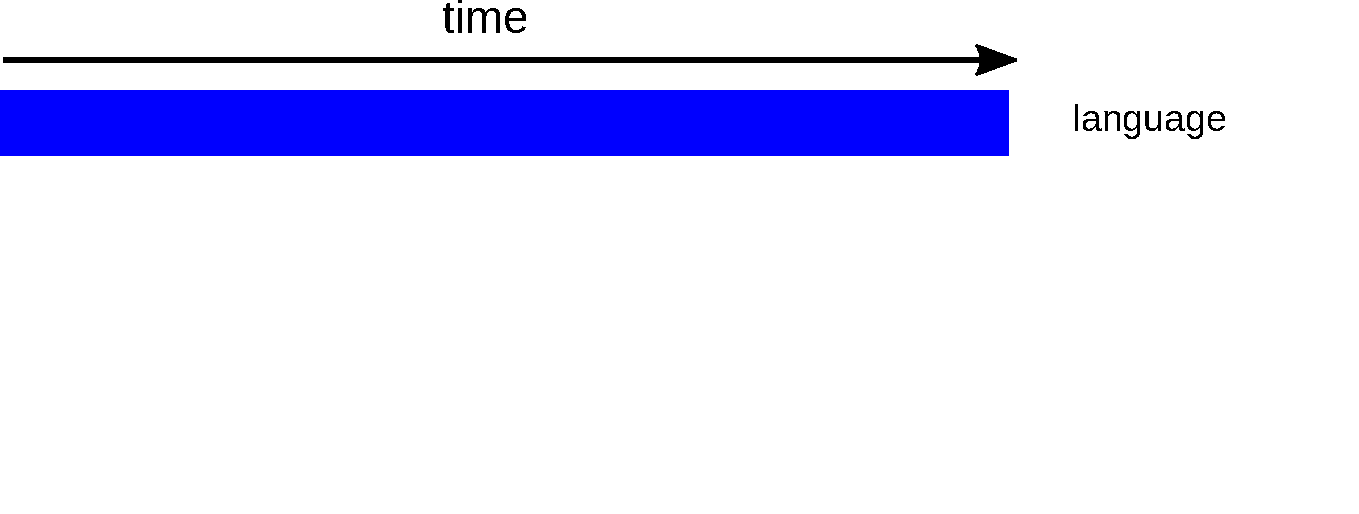
\includegraphics[width=\textwidth]{nochange.pdf}\vfill ~
}


\frame{
\vspace*{1cm}
\frametitle{Internal change}
  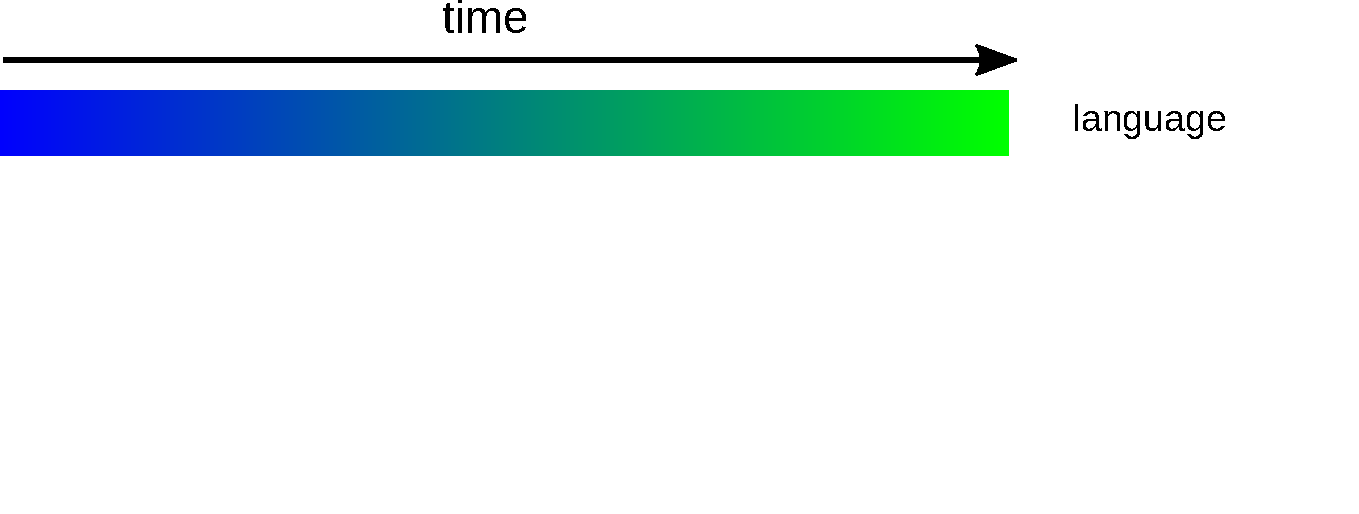
\includegraphics[width=\textwidth]{internalchange.pdf}\vfill ~
}


\frame{
\vspace*{1cm}
\frametitle{Contact-induced change }
  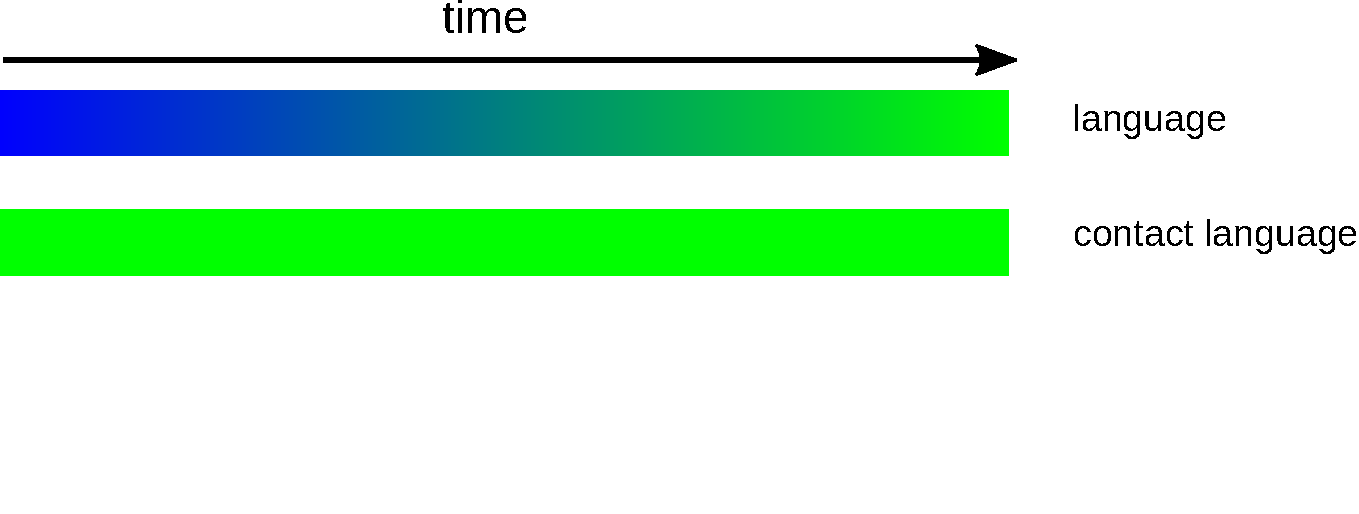
\includegraphics[width=\textwidth]{contactinducedchange.pdf}\vfill ~
}


\frame{
\vspace*{1cm}
\frametitle{Contact-induced non-change}
  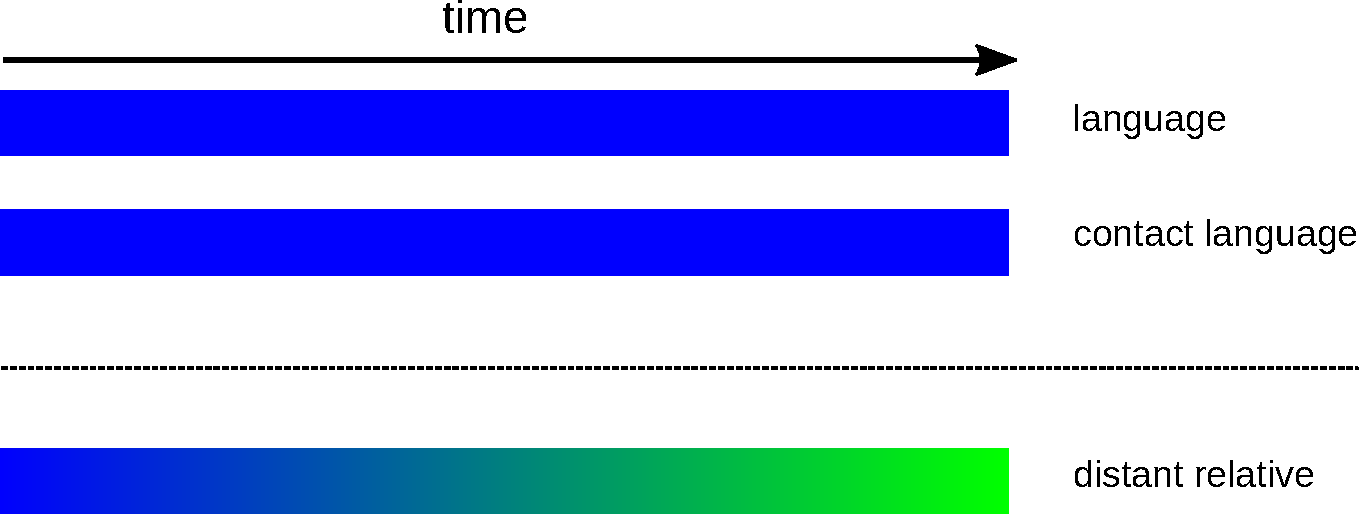
\includegraphics[width=\textwidth]{contactinducednonchange.pdf}\vfill ~
}


\frame{
\vspace*{1cm}
\frametitle{Contact-induced reversal:\\cover-up\strut}
  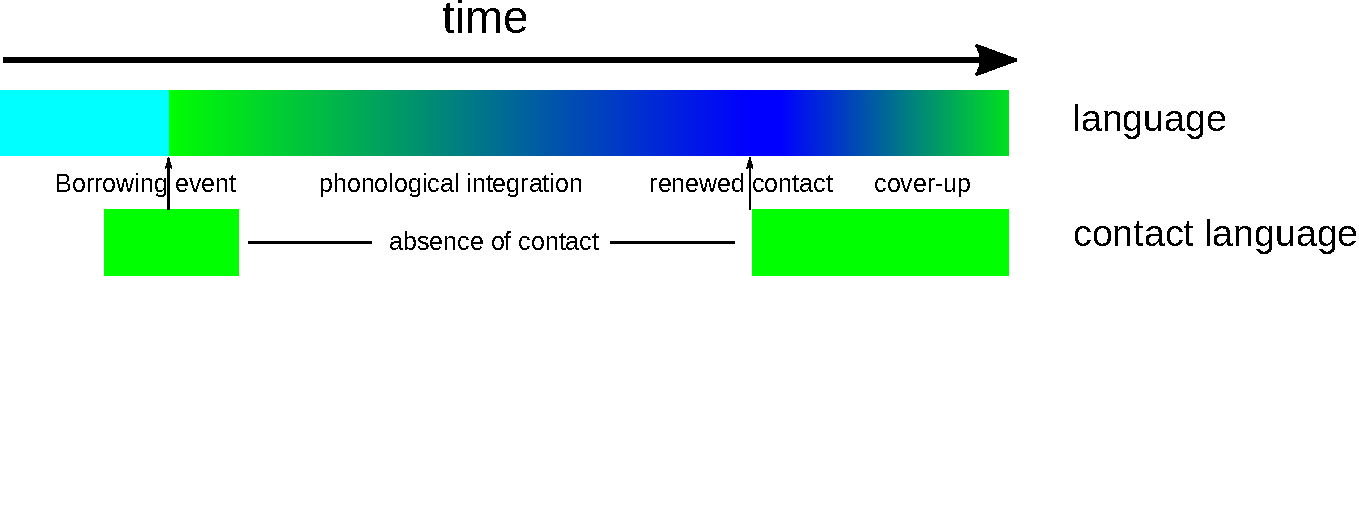
\includegraphics[width=\textwidth]{contactreversal.pdf}

\vspace*{-10mm}
  \begin{itemize}
    \item A loandword (green) is borrowed
    \item becomes phonologically integrated (blue) when contact ceases
    \item upon renewed contact, the phonological integration is undone
  \end{itemize}\vfill ~
}

\section{The setting}

\frame{
\frametitle{The setting}
  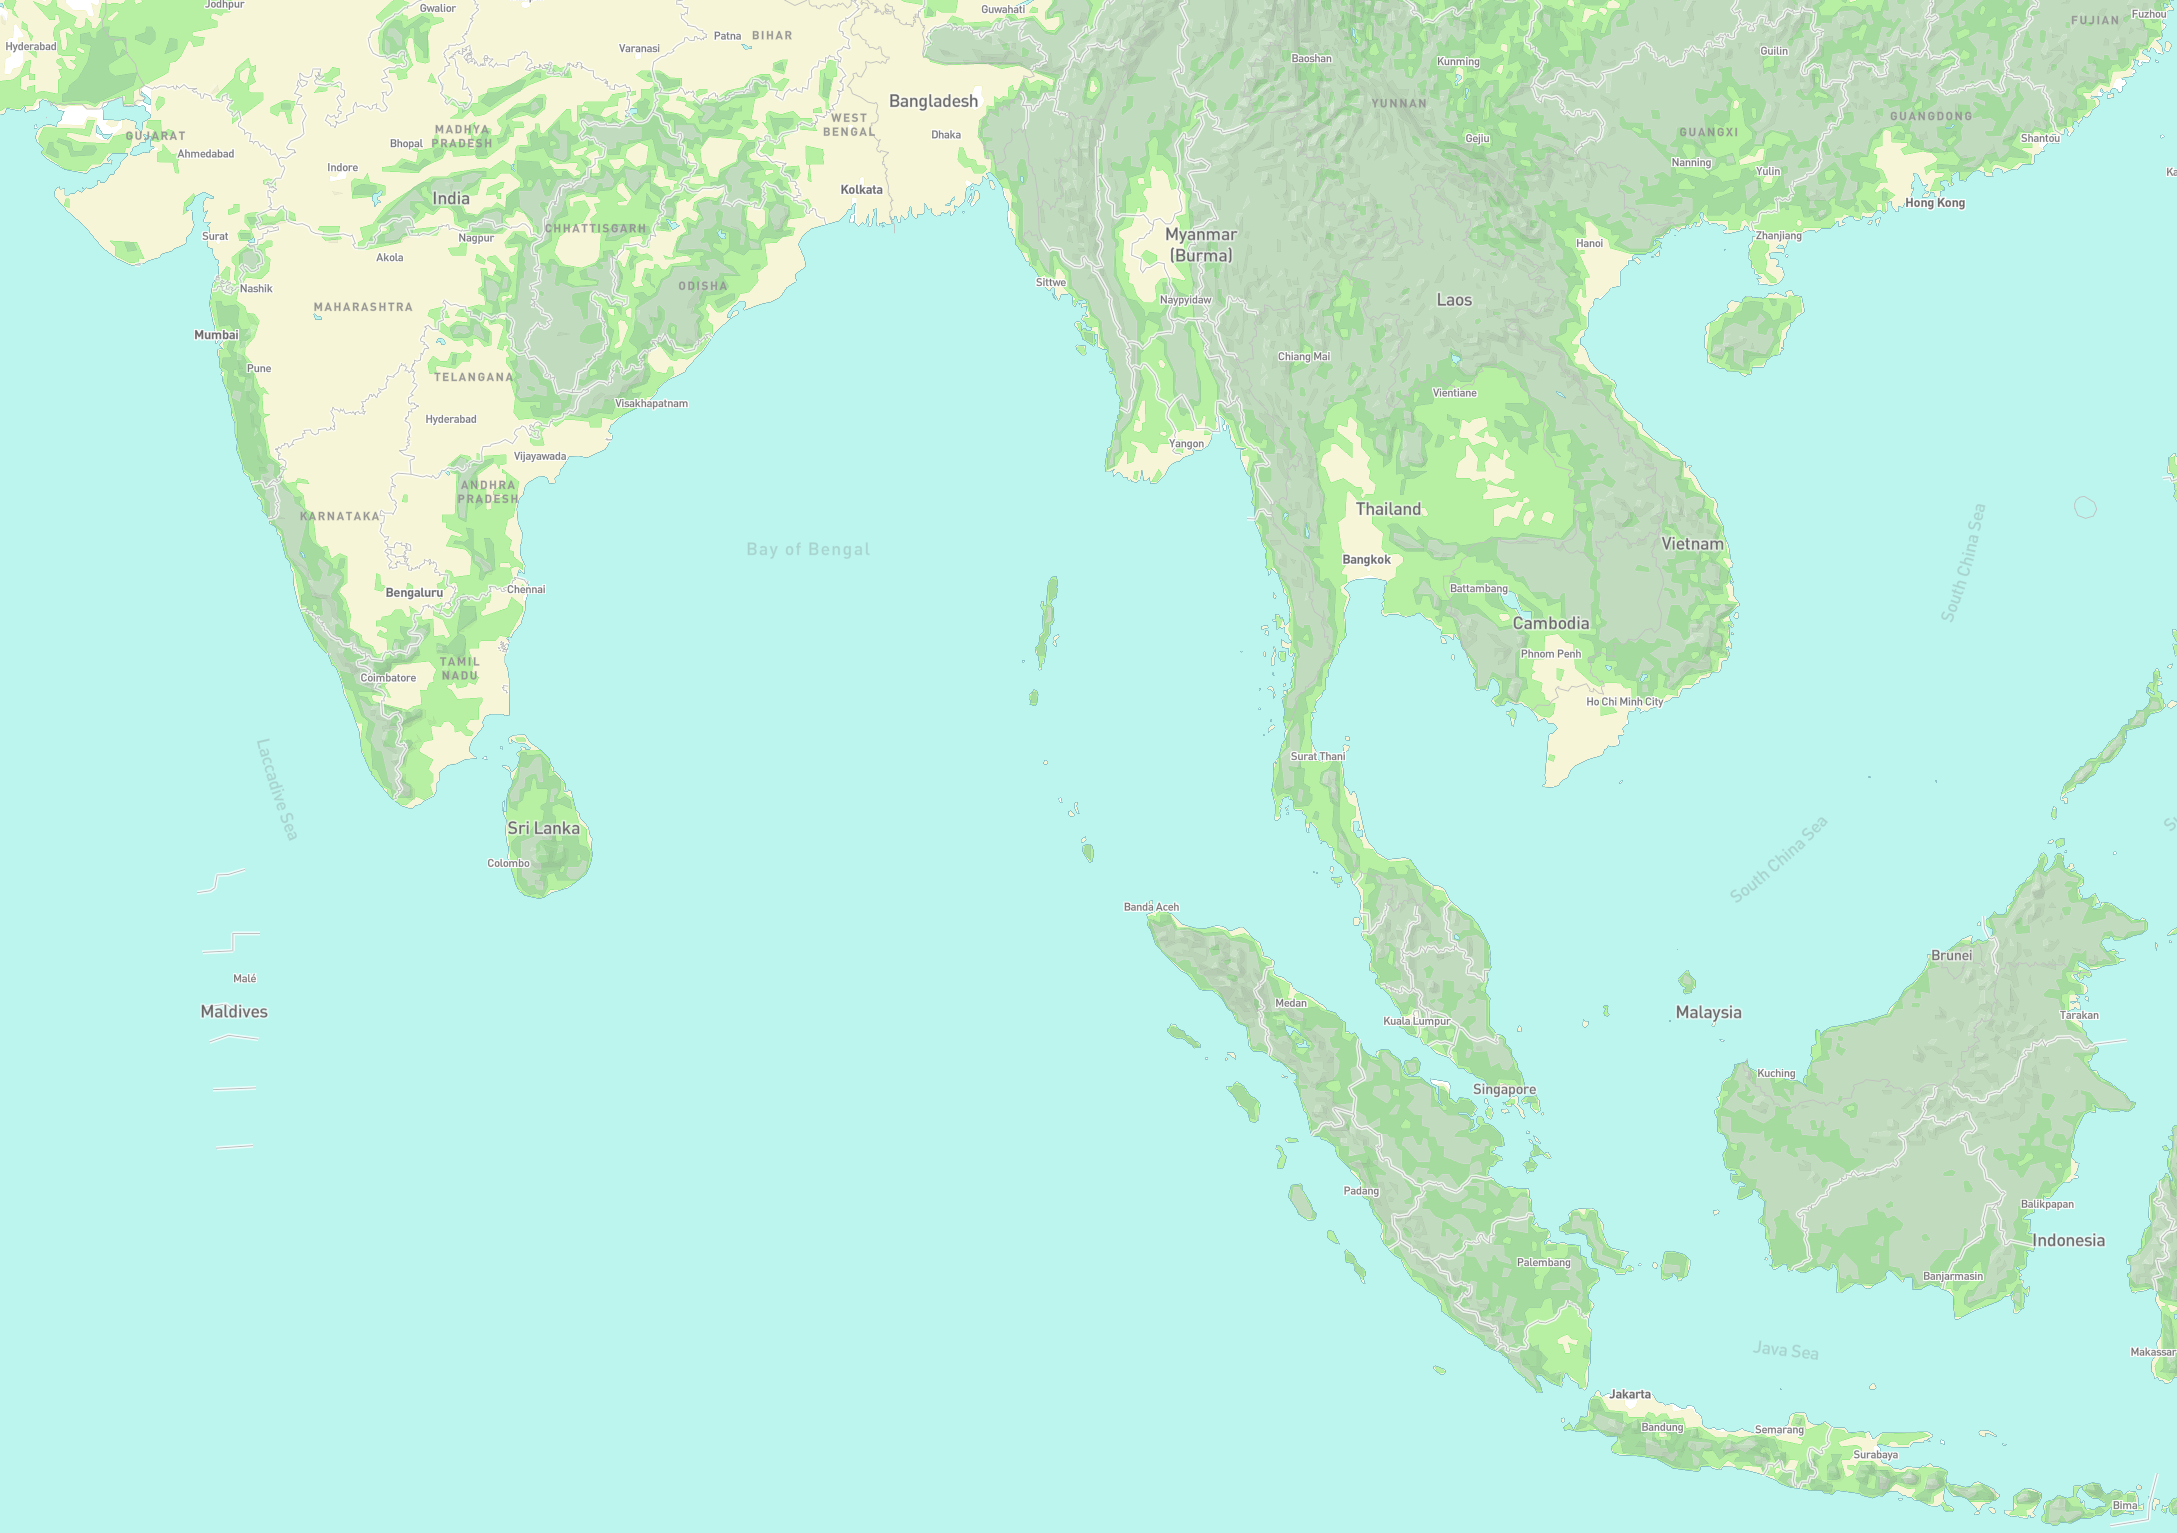
\includegraphics[width=\textwidth]{bayofbengal.png}
}

\frame{
\frametitle{The setting}
 \begin{itemize}
    \item Either side of the Bay of Bengal
    \item In the West: South Asian Sprachbund \citep{Masica1976}
    \item In the East: the Malysian peninsula and archipelago
    \item long standing trade relations
    \item precolonial language contact
    \item loanwords from
    \begin{itemize}
      \item Hindi  \citep{Hamilton1919} % https://www.jstor.org/stable/41561311
      \item Tamil, from at least 900 CE \citep{Hoogervorst2015}
      \item other Indian languages  \citep{Jones2007}
    \end{itemize}
  \end{itemize}
}



\section{Comparison}
\frame{
\frametitle{Phonological comparison}
\begin{tabular}{ll}
\toprule
Indian sprachbund & Malay world \\
\midrule
     two coronal places of articulation    &     one coronal place of articulation   \\
         ~~dental                            &                                         \\
         ~~retroflex                         &                                         \\
\tablevspace
     vowel length                          &     no distinctive vowel length         \\
\tablevspace
     geminate consonants                   &     no distinctive consonant length     \\
\tablevspace
     aspirated consonants                  &     no aspirated consonants             \\
\bottomrule
\end{tabular}
}


\section{Indian loanwords in Malay}

\frame{
\frametitle{Indian loanwords in Malay}
  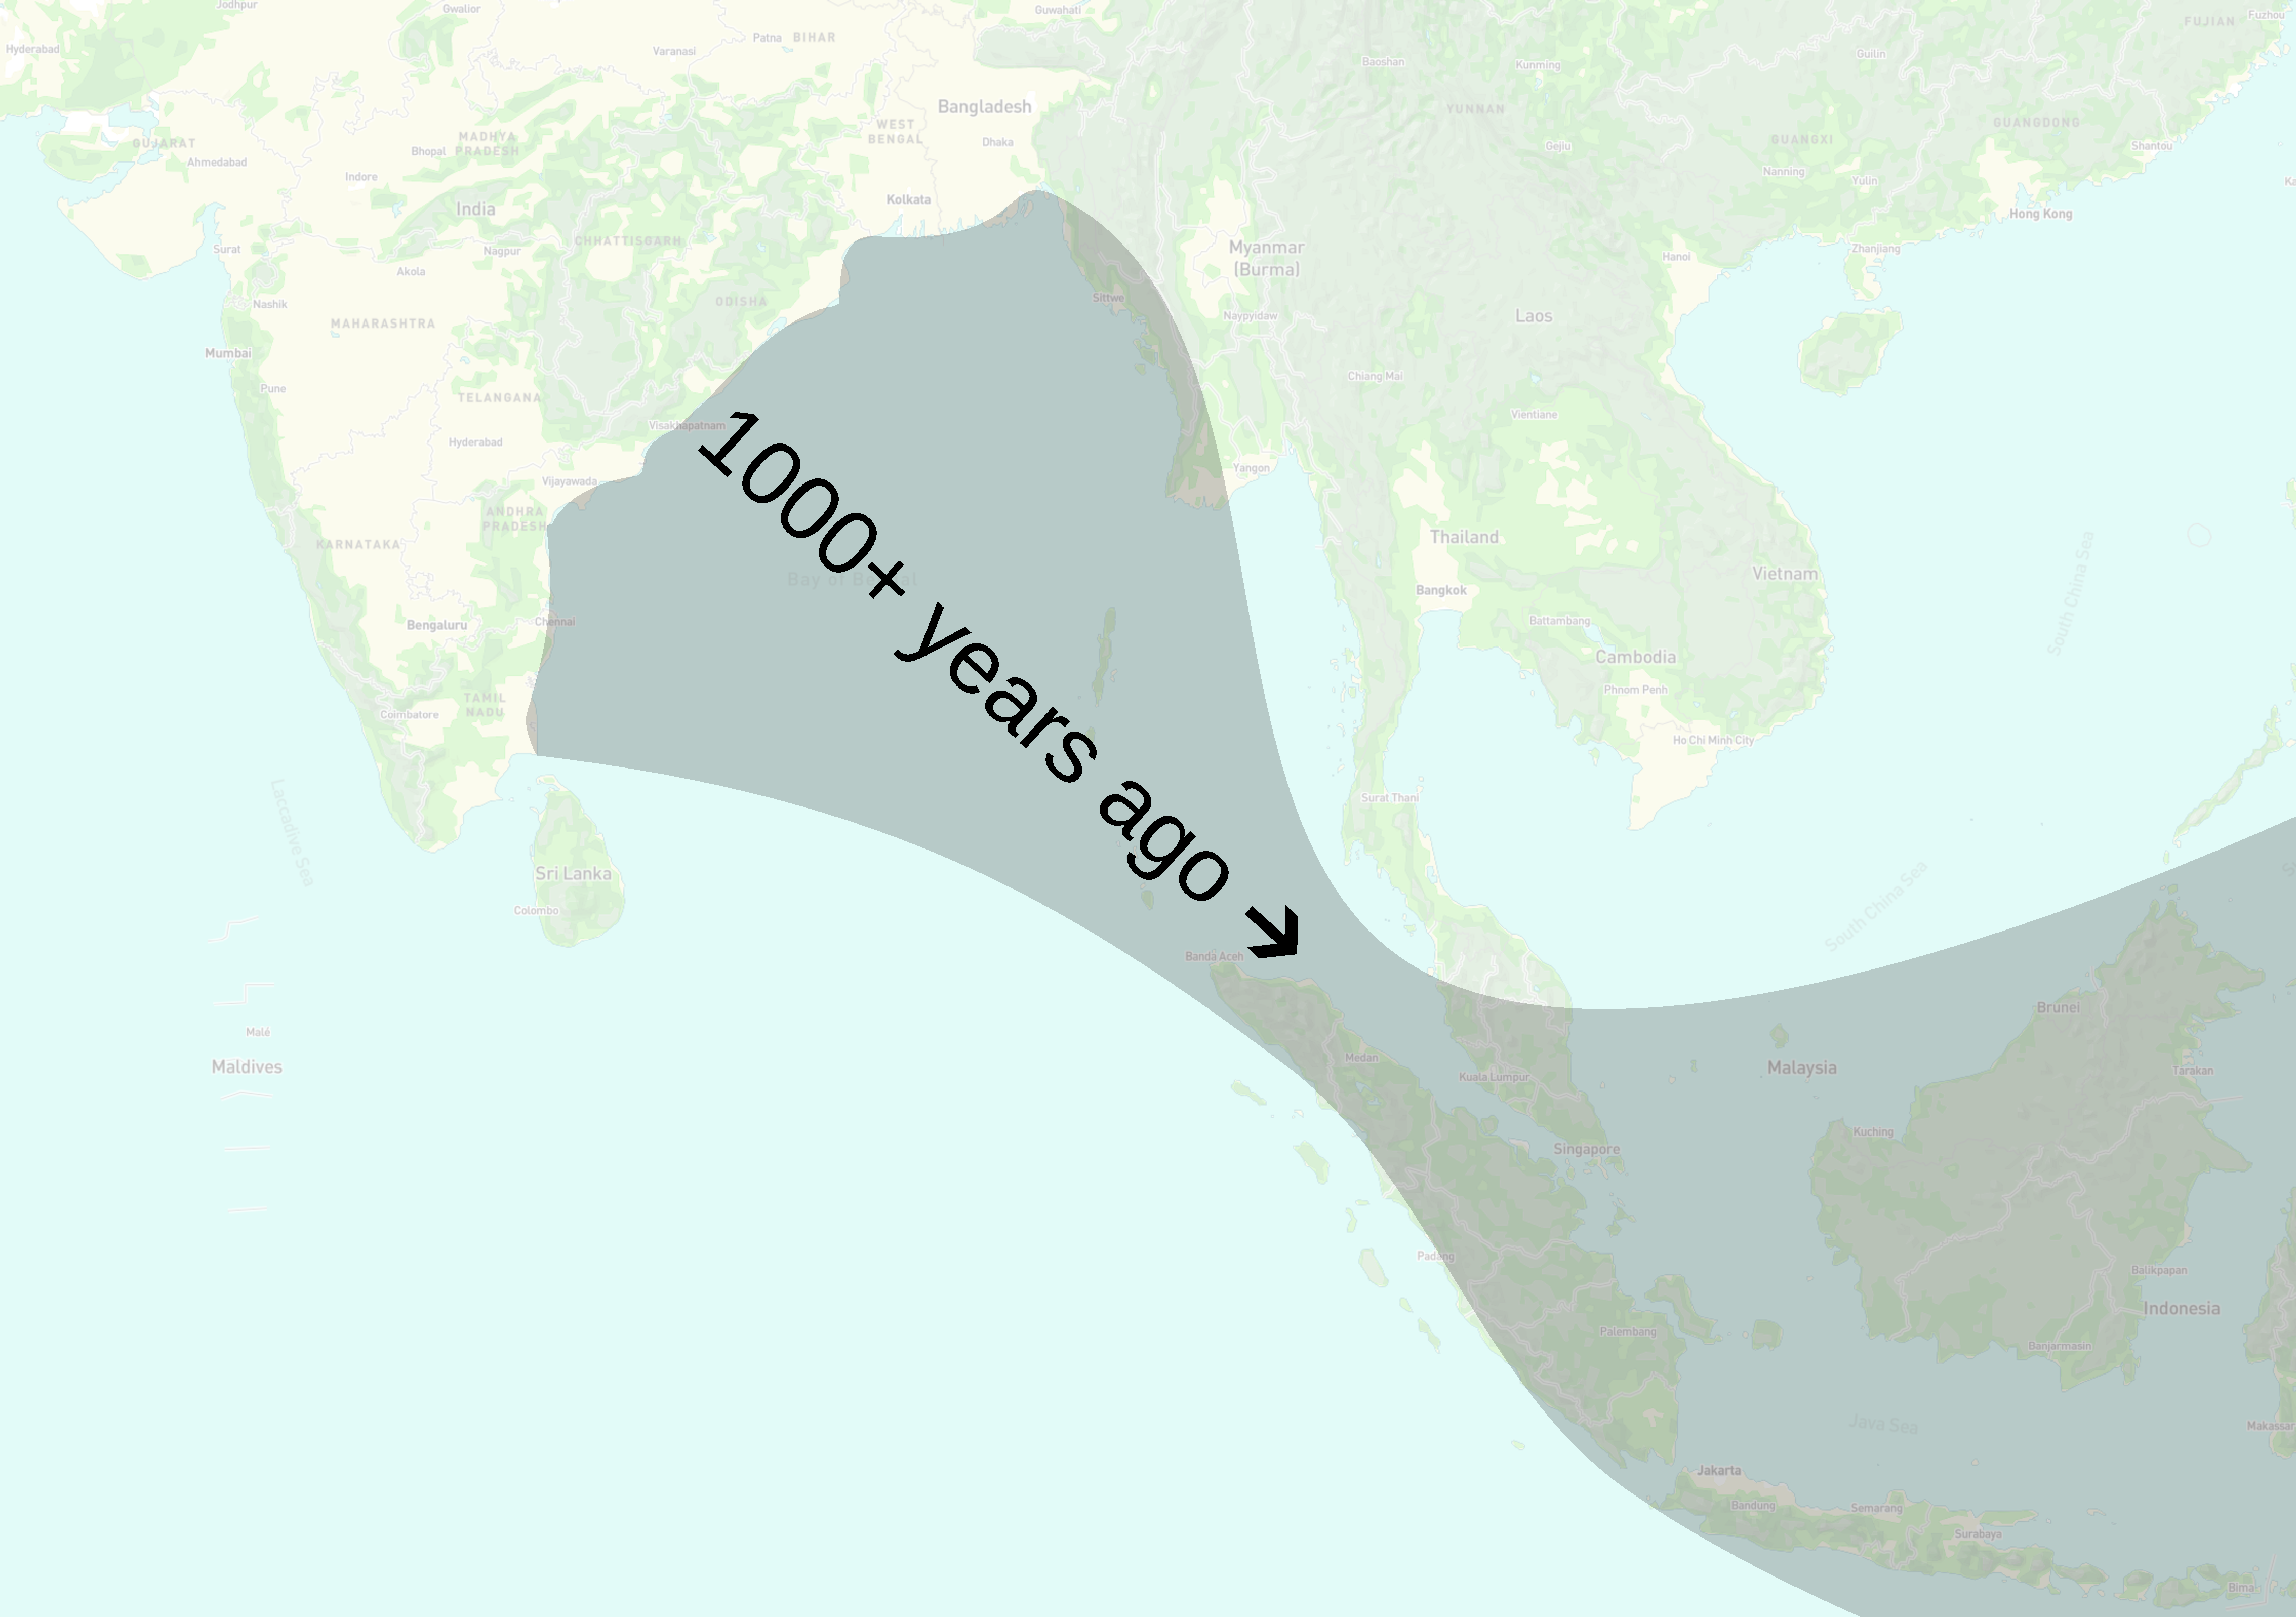
\includegraphics[width=\textwidth]{bayofbengal1000.pdf}
}

\frame{
\frametitle{Indian loanwords in Malay}
 \begin{itemize}
    \item     predictably lose their Indian features
    \item     phonological integration
    \begin{itemize}
    \item     \textit{kathā} $\to$ \textit{kata} `word'
      \begin{itemize}
        \item loss of aspiration, vowel length
      \end{itemize}
    \item     \textit{bhāṣā} $\to$ \textit{bahasa} `language'
      \begin{itemize}
        \item split of aspiration, vowel length, fronting of retroflex sibilant
      \end{itemize}
    \item     \textit{kaṭṭil} $\to$ \textit{katil} `bed'
      \begin{itemize}
        \item degemination, fronting of retroflex stop
      \end{itemize}
    \end{itemize}
    \item     \citet{Hamilton1919,Jones2007,Hoogervorst2015}
 \end{itemize}
}





\section{Sri Lanka Malay}
\frame{
\frametitle{Sri Lanka Malay}
 \begin{itemize}
    \item   language of the ethnic group of Malays in Sri Lanka
    \begin{itemize}
      \item 46,000 Malays in Sri Lanka (0.3\% of the population)
    \end{itemize}
    \item   brought between roughly 1650 and 1850
    \begin{itemize}
      \item colonial powers of the Dutch and the British
      \item exiles
      \item mercenaries
      \item slaves
    \end{itemize}
    \item   contact languages Sinhala (Indo-Aryan) and Tamil (Dravidian)
    \item   important language change with phenomenal speed ensues
    \item \citet{Hussainmiya1990,Nordhoff2009phd,NordhoffEd2012Brill}
  \end{itemize}
}

\frame{
\frametitle{\mbox{Migration of Malays to Sri Lanka}}
  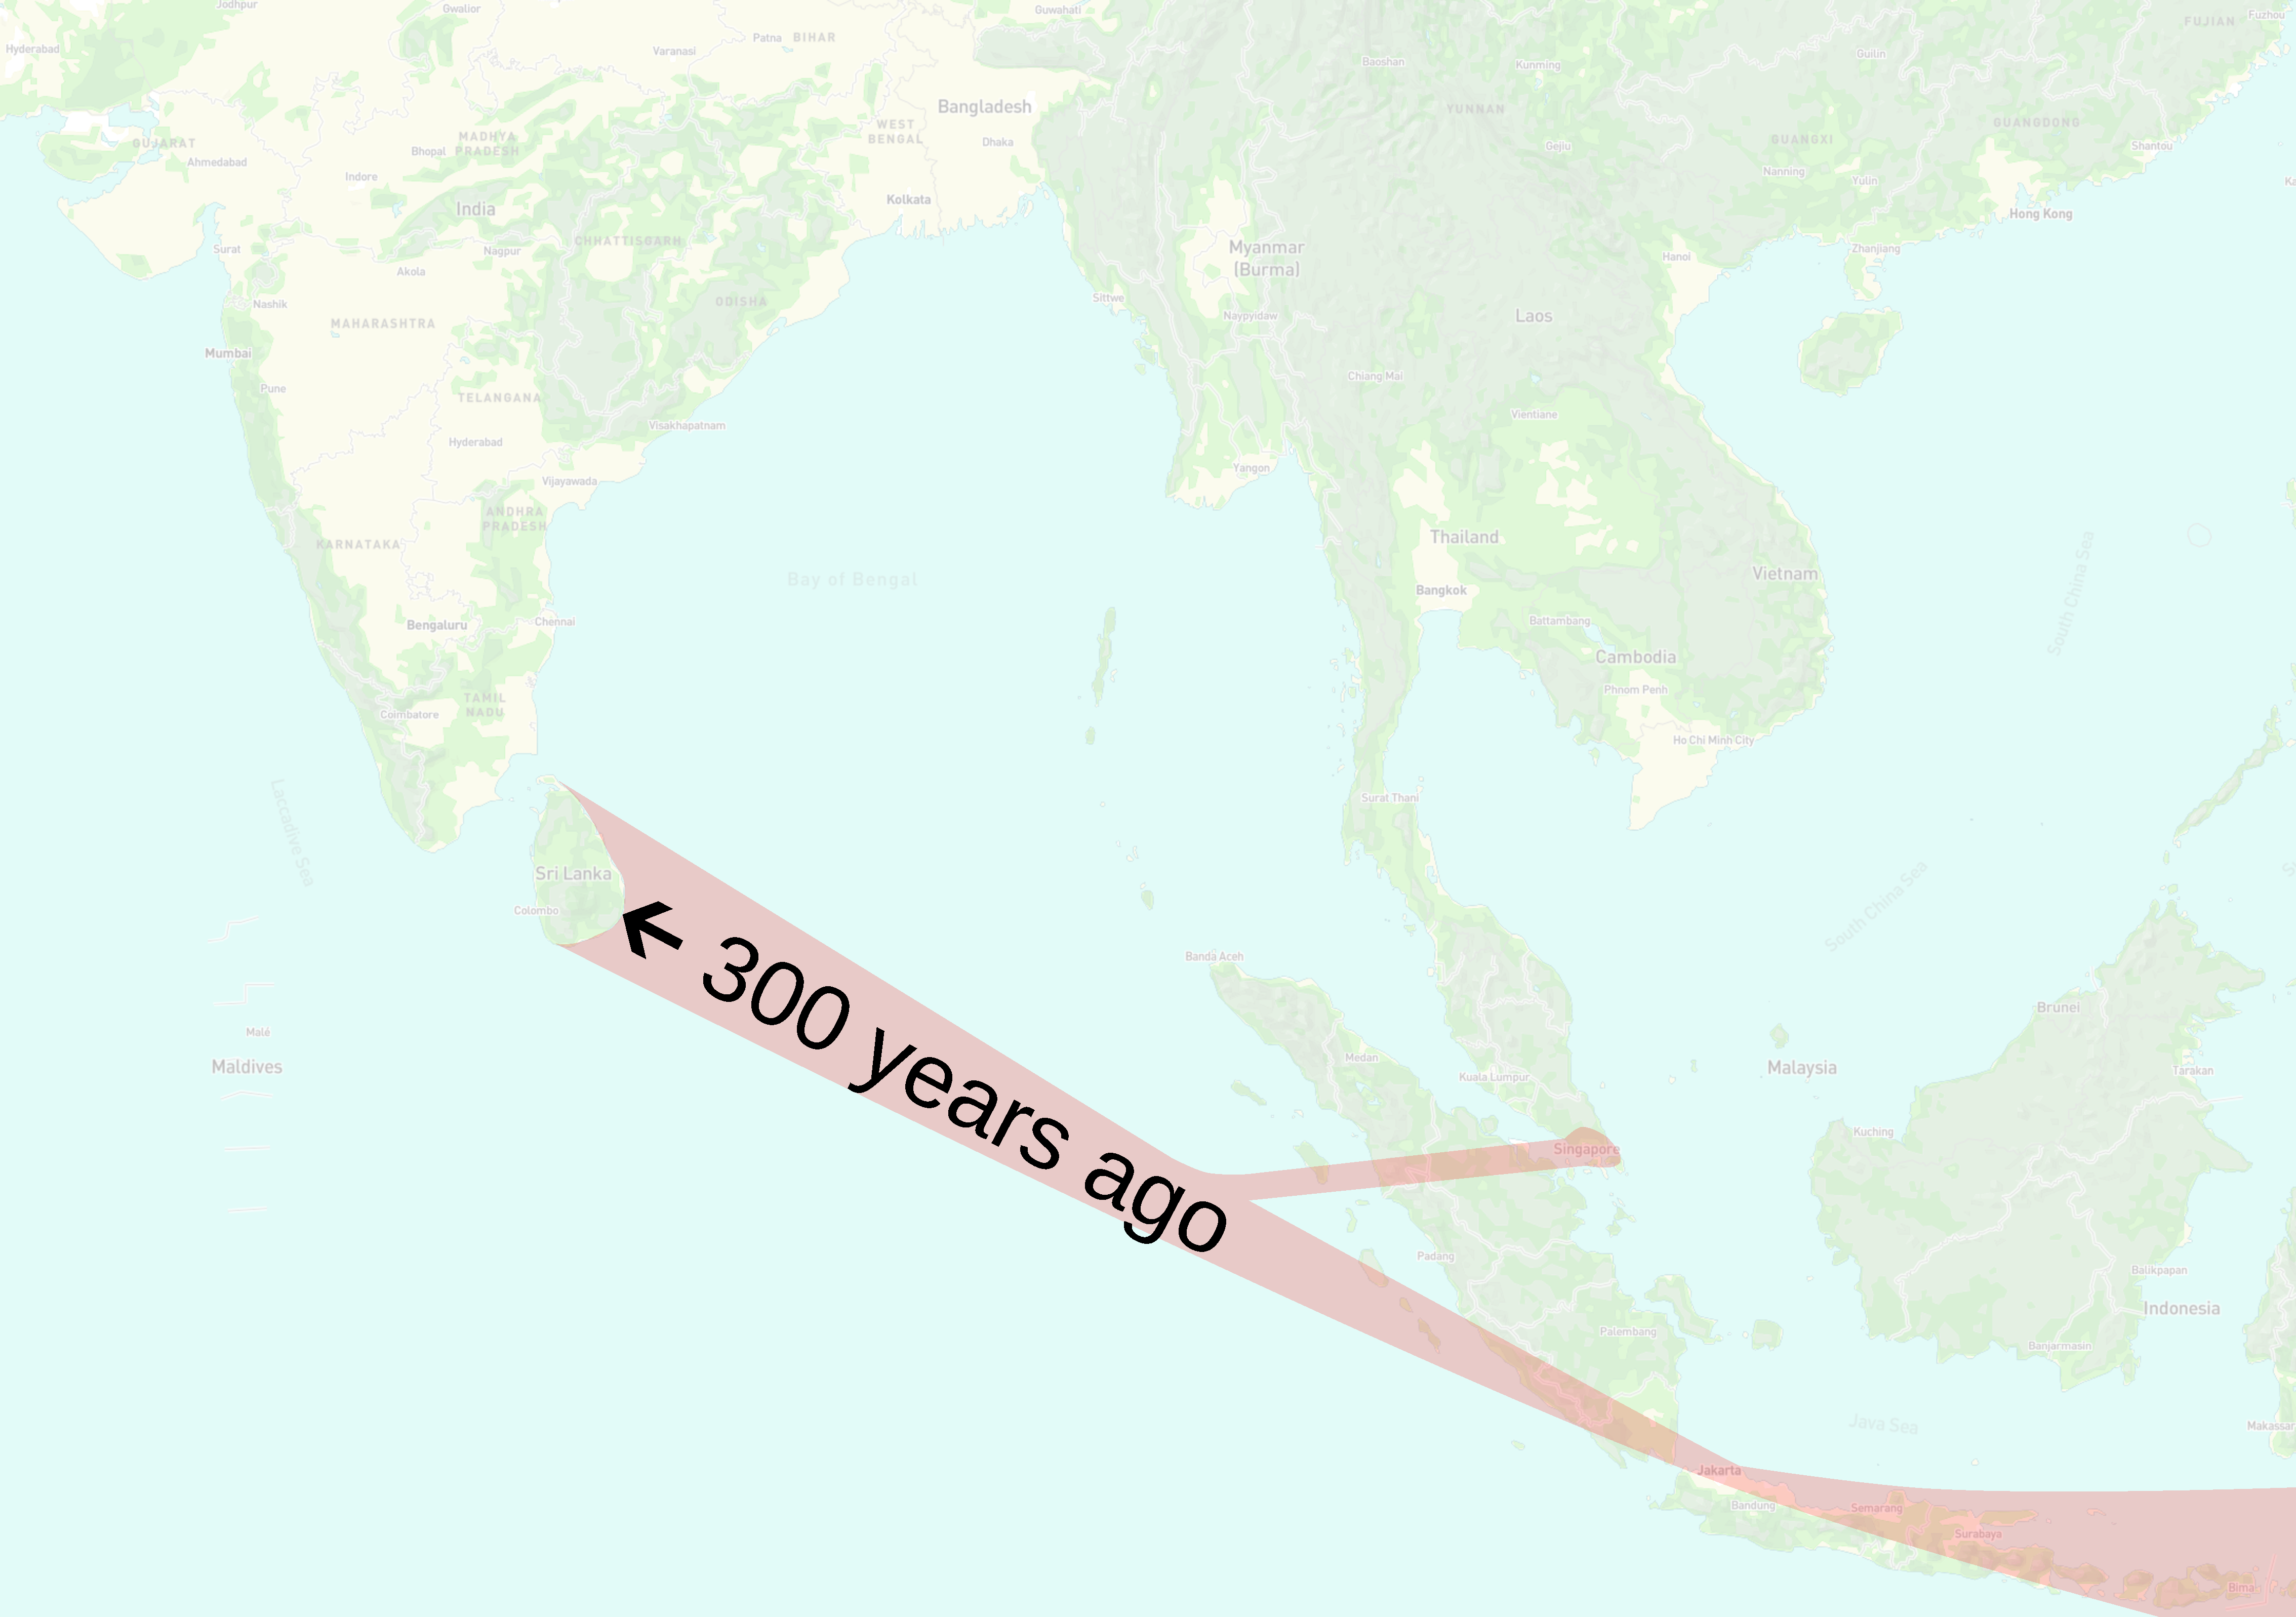
\includegraphics[width=\textwidth]{bayofbengal300.pdf}
}



\frame{
\frametitle{Language contact:\\ new features}
  \begin{itemize}
    \item syntax
    \begin{itemize}
      \item       SOV word order
      \item       postpositions
    \end{itemize}
      \item morphology
      \begin{itemize}
      \item       case clitics
      \item       participles, infinitives
      \end{itemize}
    \item phonology
      \begin{itemize}
      \item       dental/retroflex distinction
      \item       vowel length/consonant length
      \begin{itemize}
      \item           depends on analysis, one is sufficient to account for the other
      \end{itemize}
    \item       prenasalized consonants
    \end{itemize}
    \item all of this is about as far away from a well-behaved Malay variety as it gets
    \item \citet{NordhoffEd2012Brill}
 \end{itemize}
}



\section{The SLM word}
\frame{
\frametitle{Metrical structure of the SLM word}
\begin{itemize}
  \item most words have two syllables
  \item the penultimate syllable typically either has a coda (CVC) or a long vowel (CVV)
  \item well-formed words
  \begin{itemize}
      \item CVV.CV
      \item CVC.CV
  \end{itemize}
  \item generalization
    \begin{itemize}
      \item CVX.CV
    \end{itemize}
   \item analysis: extrametrical final syllable with a bimoraic foot constraint
   \begin{itemize}
    \item C(V$_\mu$X$_\mu$).<CV>
    \item \citet{Nordhoff2009phd}
   \end{itemize}
 \end{itemize}
}



\section{Phonological change}
\frame{
\frametitle{Regular sound change:\newline \mbox{Vowel lengthening{\slash}gemination}}
\begin{columns}
  \column{6cm}
 \begin{itemize}
    \item     \textit{nasi} $\to$ \textit{naasi} `rice'
    \item     \textit{cuci} $\to$ \textit{cuuci} `wash'
    \item     \textit{sopi} $\to$ \textit{soopi} `liquor'
    \item     \textit{mati} $\to$ \textit{maa\textsubbridge{t}i} `to die'
    \item     \textit{derapa} $\to$ \textit{draapa} `how much'
    \item     \textit{bəsar} $\to$ \textit{bìssar}  `big'
 \end{itemize}
 \column{4cm}
 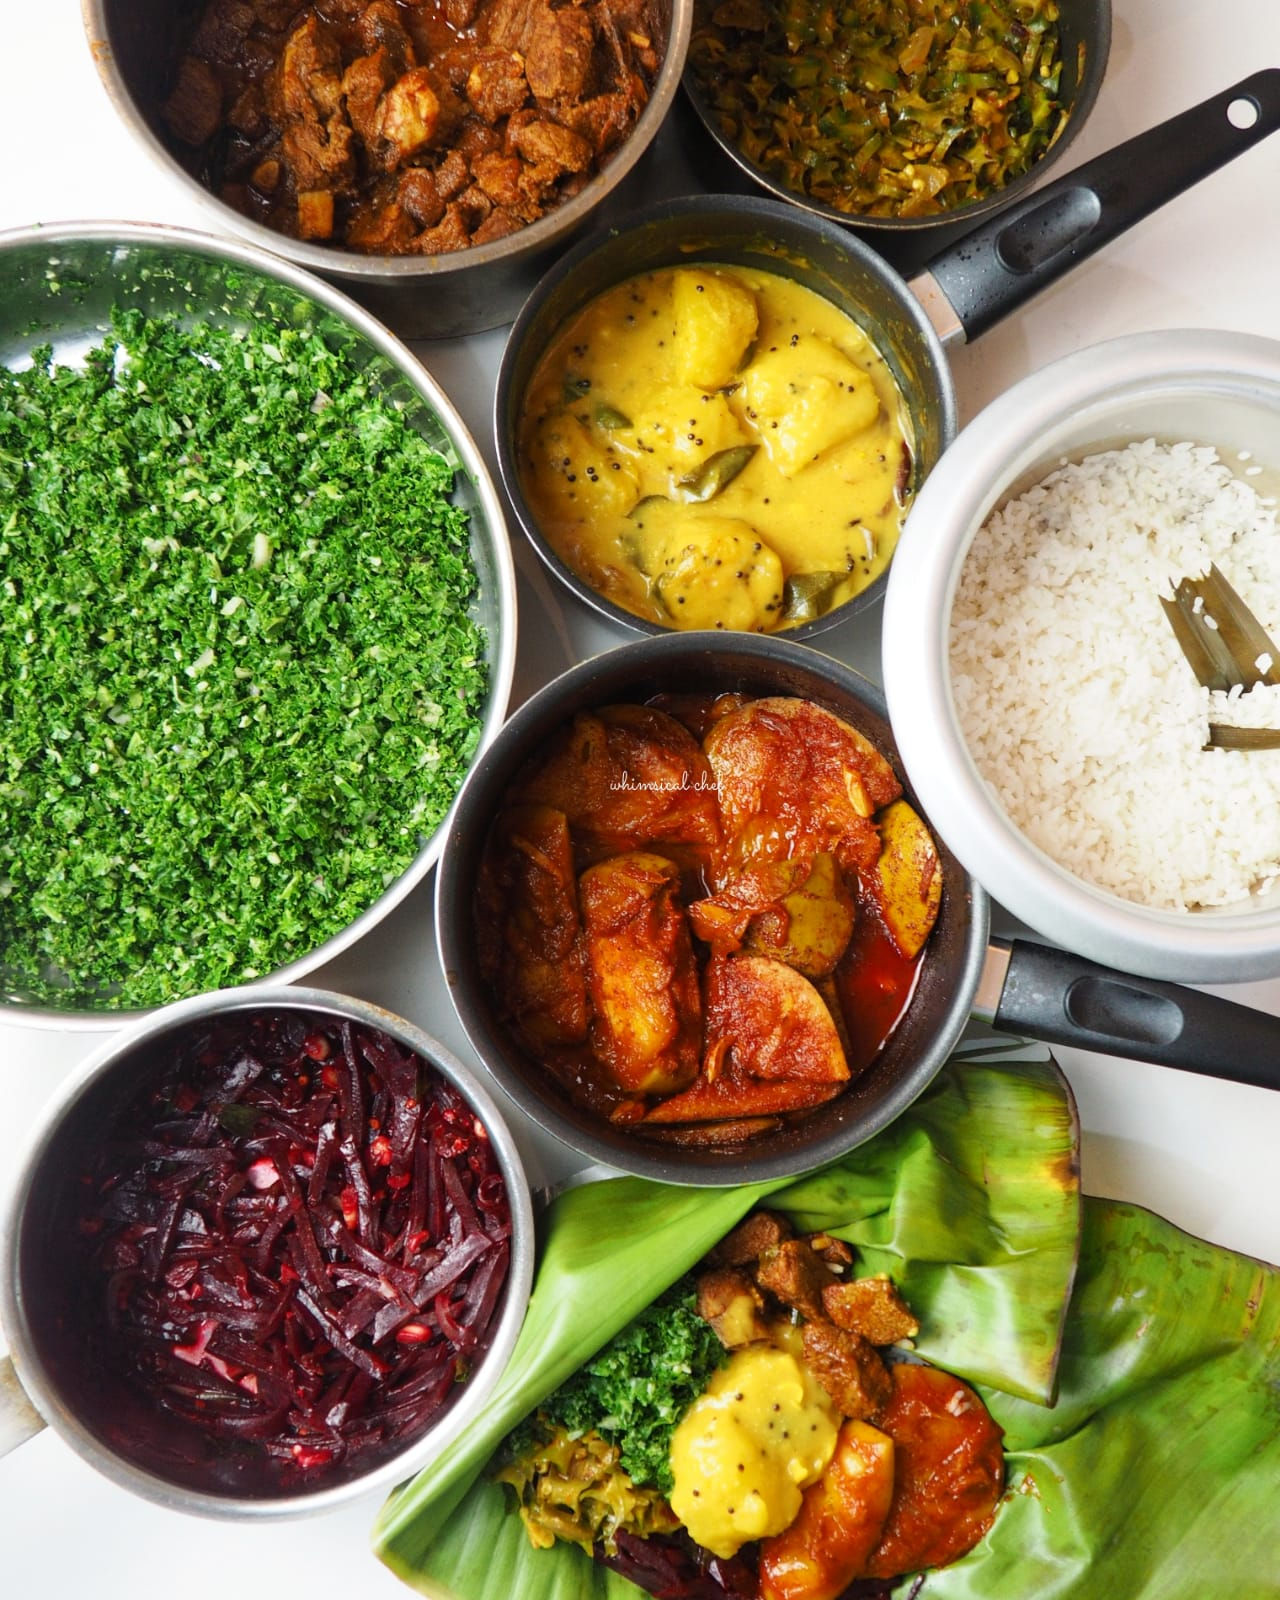
\includegraphics[width=.8\textwidth]{riceandcurry.jpg}

 {\tiny CC-BY Lankan Foodie \url{https://commons.wikimedia.org/wiki/File:Sri_Lankan_Rice_and_Curry.jpg}}
\end{columns}
}



\frame{
\frametitle{Exceptions to regular sound change}
\begin{columns}
\column{6cm}
 \begin{itemize}
    \item   expected
    \begin{itemize}
      \item       \textit{kapal} $\to$ \textit{*kaapal} `ship'
      \item       \textit{topi} $\to$ \textit{*\textsubbridge{t}oopi} `hat'
      \item       \textit{katil} $\to$ \textit{*kaa\textsubbridge{t}il} `bed'
    \end{itemize}
    \item   found
    \begin{itemize}
    \item       \textit{kapal} $\to$ \textit{kappal}
    \item       \textit{topi} $\to$ \textit{\textsubbridge{t}oppi}
    \item       \textit{katil} $\to$ \textit{kaṭṭil}
    \end{itemize}
 \end{itemize}
\column{4cm}
 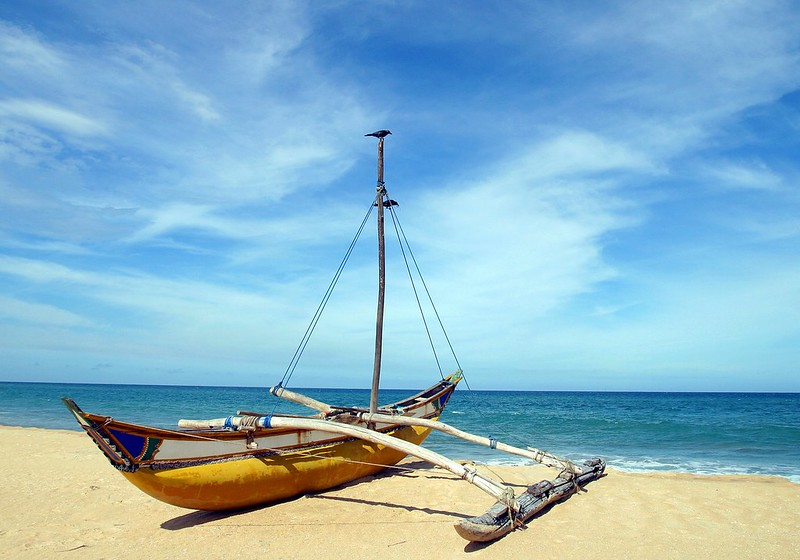
\includegraphics[width=\textwidth]{ship.jpg}
{\tiny CC-BY-NC-SA
WHL Travel
\url{https://www.flickr.com/photos/whltravel/4376067519}
}
 \end{columns}
 }



\frame{
\frametitle{No phonological cues}
 \begin{itemize}
    \item  \textit{topi/sopi} would be expected to behave alike
    \item  \textit{drapa/kapal} would be expected to behave alike
    \item  \textit{katil/mati} would be expected to behave alike
    \item  phonological conditioning unlikely
    \item  lexical specification
    \begin{itemize}
    \item      reason:  cognates in contact languages
    \item Tamil \textit{toppi, kappal, kaṭṭil}
    \item Sinhala \textit{toppiya} `hat (sg)', \textit{toppi} `hat (pl)'
    \end{itemize}
    \item  \textbf{``phonological cover-up''}
    \item the degemination undergone is undone and we find ``regemination''
 \end{itemize}
}


\frame{
\frametitle{Cover-up beyond\\ vowel lengthening}
 \begin{itemize}
    \item The preceding examples have been chosen because they are easy to grasp
    \item Could be explained as a straight new act of borrowing
    \item unlikely for high frequency concepts like BOAT, HAT, and BED
    \begin{itemize}
      \item no evidence for lexical gaps or functional differentiation
      \item one would have to argue that the word \textit{kapal} `boat' was temporarily lost on an island nation surrounded by sea, only to be subsequently reborrowed as \textit{kappal}
    \end{itemize}
    \item other, more involved domains of cover-up to be discussed now:
    \begin{enumerate}\stepcounter{enumi}
    \item  \textbf{syllabification of ŋ}
    \item  \textbf{tautosyllabic N\textsubwedge{C} clusters}
    \item  \textbf{re-fronting of voiced coronal stop}
%     \item unlengthening  of /u/
    \end{enumerate}
    \end{itemize}
    }

\frame{
\frametitle{Syllabification of ŋ}
\begin{columns}
\column{4cm}
  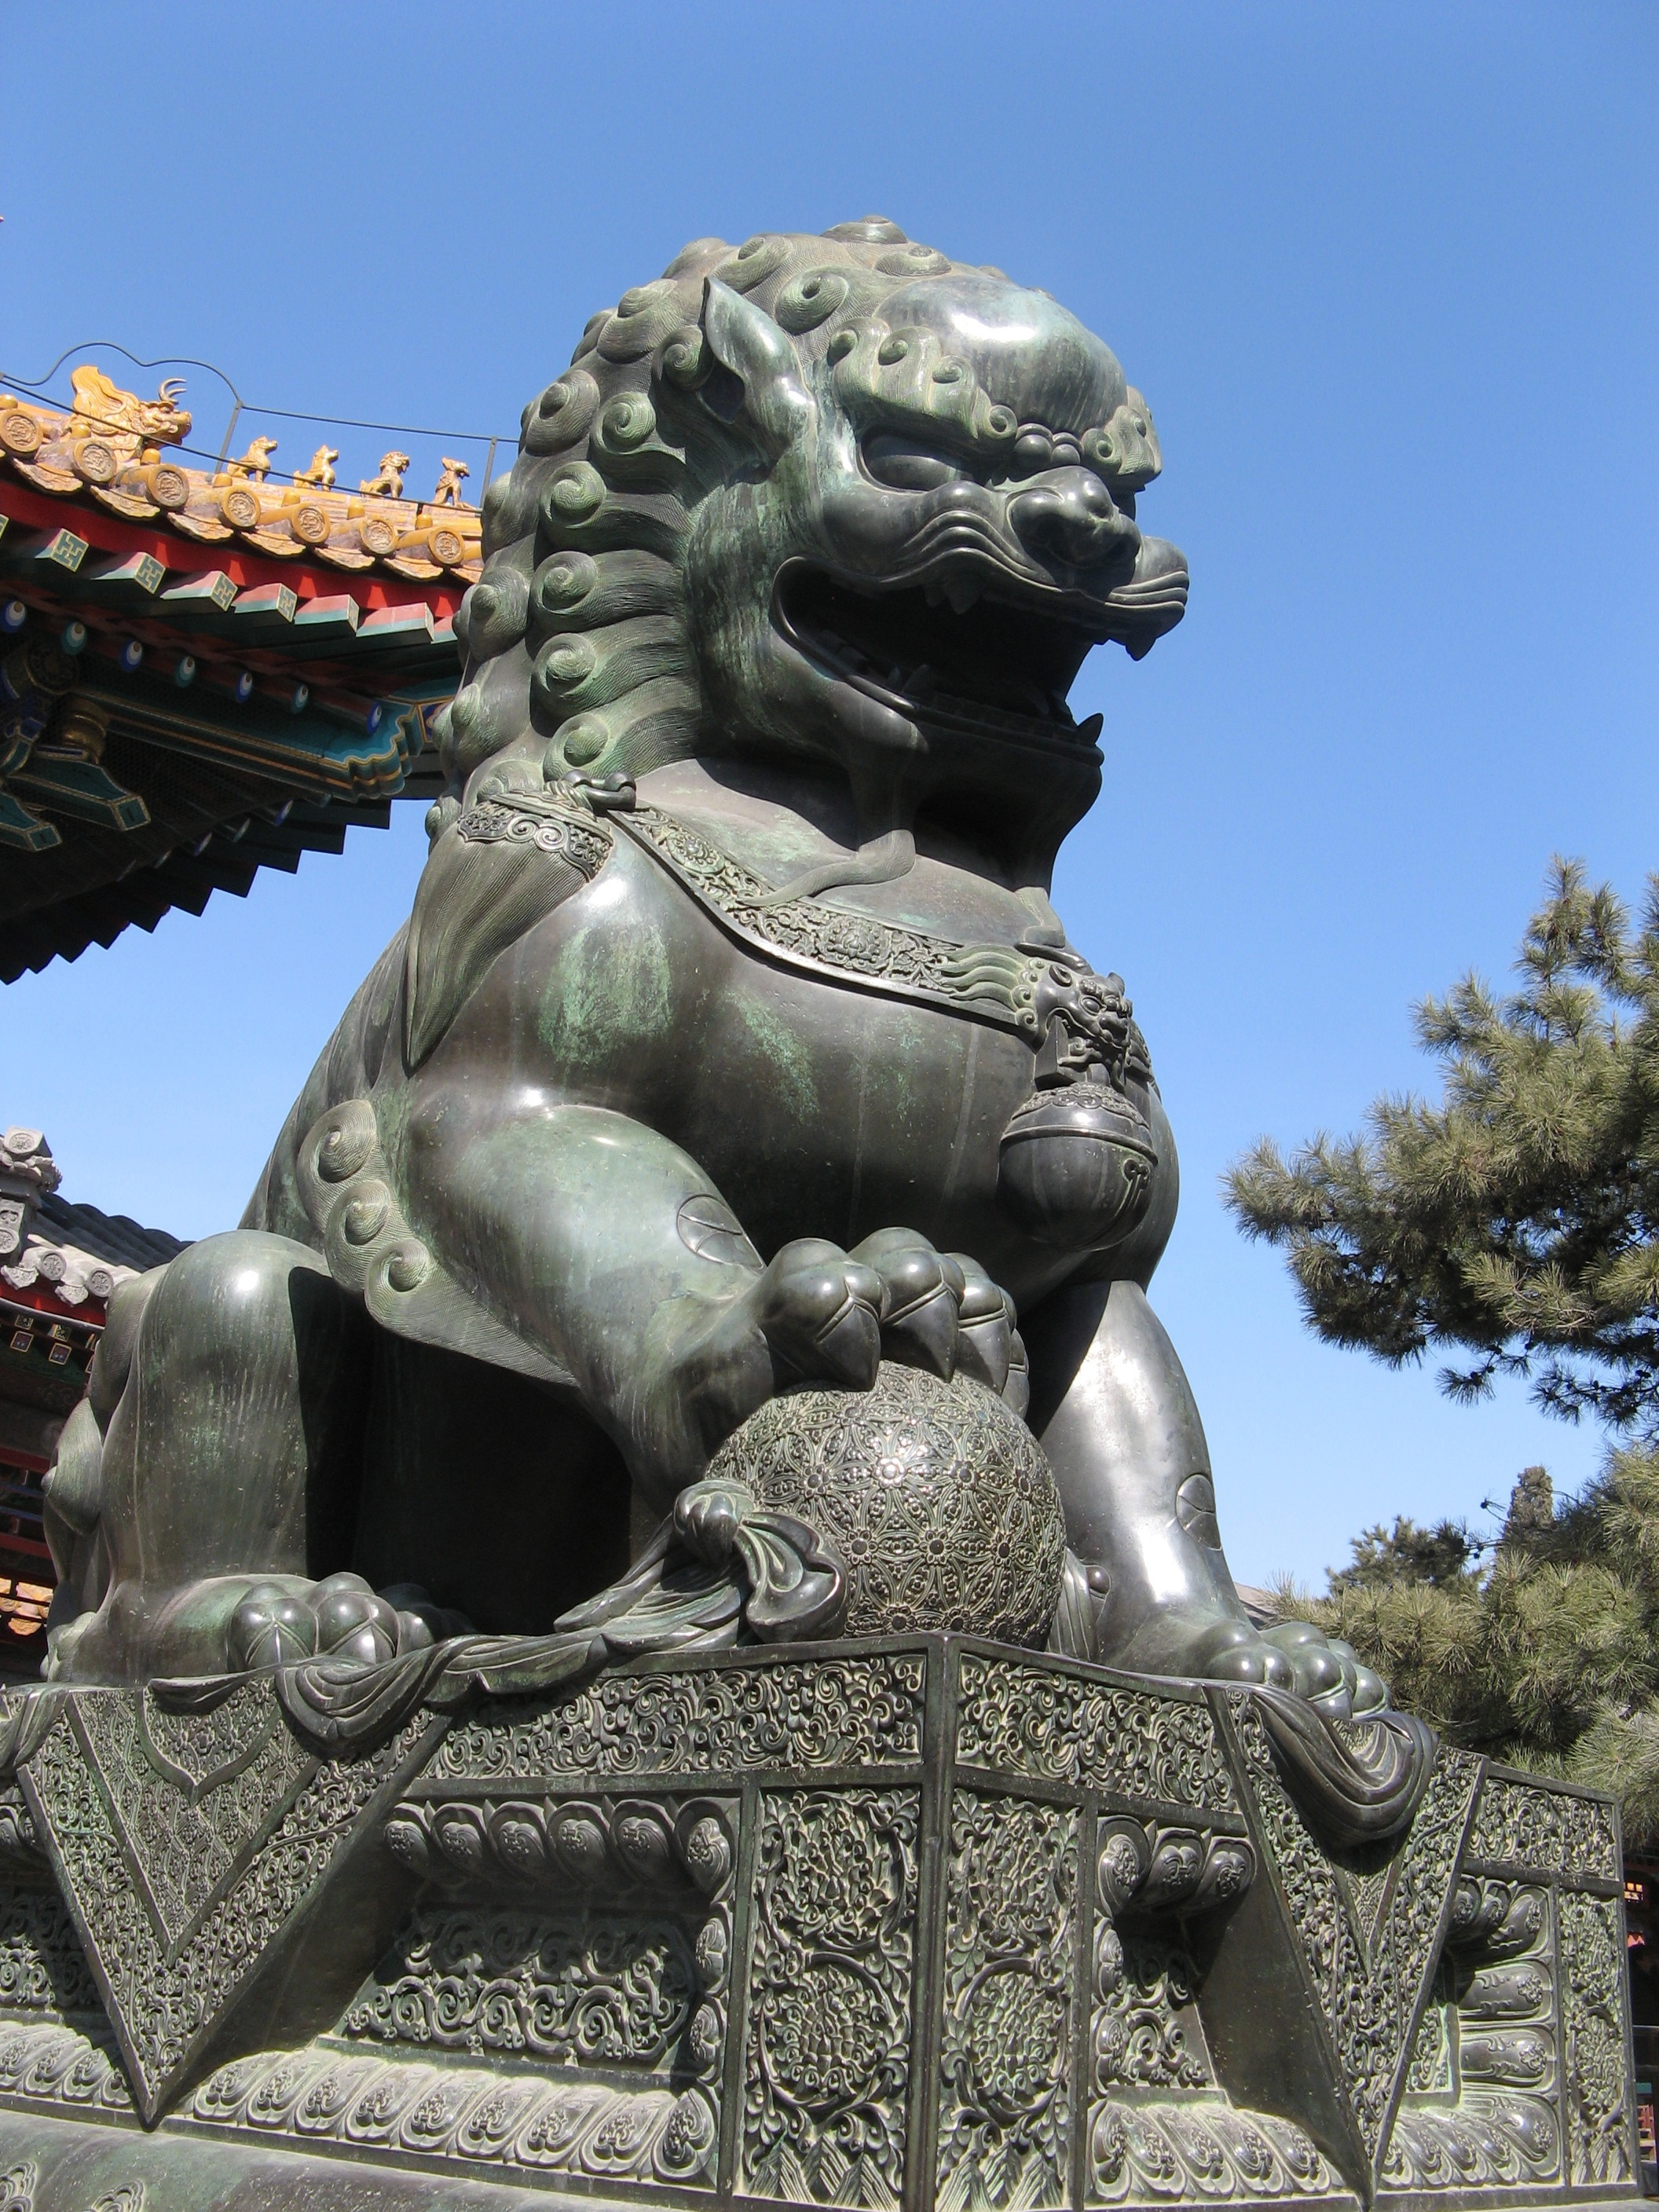
\includegraphics[height=6cm]{lion.jpg}
\column{6cm}
\begin{itemize}
  \item Malay varieties can have syllable initial ŋ
  \item So can Sri Lanka Malay
  \begin{itemize}
    \item      \textit{i.ŋat} $\to$ \textit{ii.ŋa\textsubbridge{t}} `to think'
   \end{itemize}
  \item based on this, we would expect \textit{si.ŋa} $\to$ \textit{*sii.ŋa} `lion'
  \item but we get
  \begin{itemize}
    \item      \textit{si.ŋa} $\to$ \textit{siŋ.ga}
  \end{itemize}
  \item the ŋ is on the left side of the syllable boundary where we would have expected the right side.
  \end{itemize}
\end{columns}
  }

\frame{
\frametitle{Syllabification of ŋ}
\begin{itemize}
  \item explanation: Sinhala \textit{siŋ.ha.yaa} and Tamil \textit{ciŋ.gam} with a velar nasal coda in the first syllable
  \begin{itemize}
  \item Sanskrit \textit{siṃ.há} %, Hindi \textit{siṅgh}\\
  ~~~~$\downarrow$
  \item resyllabification to \textit{si.ŋa} in Malay\\
  ~~~~$\downarrow$
  \item ``deresyllabfication''/cover-up in Sri Lanka Malay to \textit{siŋ.ga}
  \end{itemize}
 \end{itemize}
}

\frame{
\frametitle{N\textsubwedge{C} clusters}
 \begin{itemize}
    \item   N\textsubwedge{C} clusters with a voiced stop predictably have tautosyllabic rendering in SLM  (V.N\textsubwedge{C}V)
    \begin{itemize}
    \item       \textit{gam.bar} $\to$ \textit{gaa.mbar} `picture'
    \item \textit{ban.jir} $\to$ \textit{baa.njir} `flooding'
  \end{itemize}
  \hspace*{6cm}{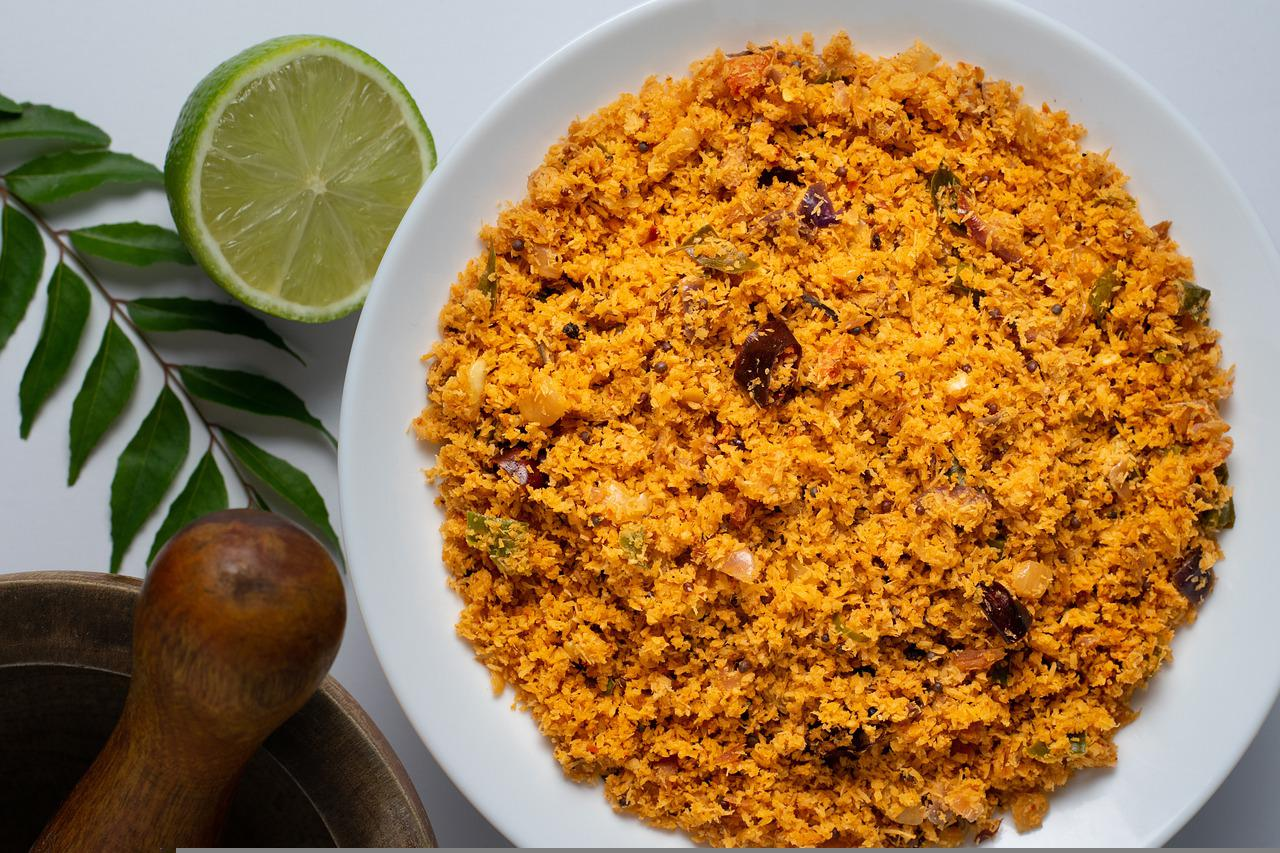
\includegraphics[width=4cm]{sambol.jpg}\vspace*{-2.7cm}}
  \item exception
  \begin{itemize}
    \item       \textit{sam.bal} $\to$  \textit{*saa.mbal} `spicy dish'
    \item       \textit{sam.bal} $\to$ \textit{sam.bal}
    \item       \textit{kan.ji} $\to$  \textit{*kaa.nji} `rice gruel'
    \item       \textit{kan.ji} $\to$ \textit{kan.ji}
  \end{itemize}
  \end{itemize}
}

\frame{
\frametitle{N\textsubwedge{C} clusters}
 \begin{itemize}
  \item explanation
  \begin{itemize}
    \item Tamil \textit{cam.bal}, Sinhala \textit{sam.bol} have heterosyllabic clusters
    \item Tamil \textit{kañ.ci}, has a  heterosyllabic cluster
    \begin{itemize}
      \item NB: all Tamil NC clusters are always heterosyllabic, but Sinhala has words with tautosyllabic clusters.
    \end{itemize}
    \item rest of the phonology is untouched
  \end{itemize}
 \end{itemize}
}

\frame{
\frametitle{Fronting of d}
 \begin{itemize}
    \item  alveolar d becomes (post)alveolar d in Sri Lanka Malay
    \begin{itemize}
      \item \textit{lada}  $\to$ \textit{laada} `pepper'
    \end{itemize}
    \item exception:
    \begin{itemize}
    \item      \textit{kalde} $\to$ *\textit{kalde} `donkey'
    \item      \textit{kalde} $\to$ \textit{kal\textsubbridge{d}e}
    \end{itemize}
    \item explanation:
    \begin{itemize}
    \item Tamil   \textit{ka\textsubdot{l}u\textsubbridge{d}ai}  has a dental \textsubbridge{d} as well
    \item rest of the phonology is untouched
    \end{itemize}
    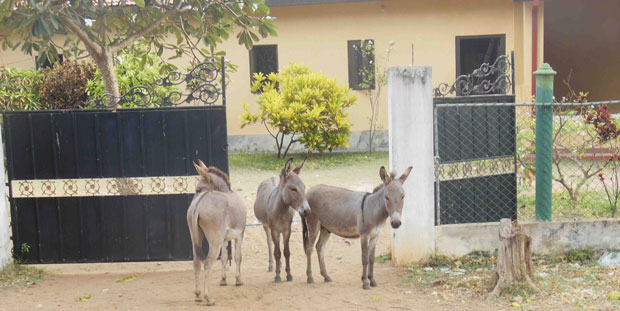
\includegraphics[width=5cm]{donkey.jpg}
 \end{itemize}
}

% \frame{
% \frametitle{other types}
%  \begin{itemize}
%     \item   (guru)
%     \item       guru $\to$ *guuru
%     \item       guru $\to$ guru
%  \end{itemize}
% }

\section{Metalinguistic awareness}
\frame{
\frametitle{Metalinguistic awareness}
 \begin{itemize}
    \item  speakers are highly multilingual and are also able to identify cognates
    \item  in order to verify my hearing of length, I regularly use Sinhala script
    \item would the word for `earth' be
    \raisebox{-2mm}{
\includegraphics[height=2em]{bumi.png}}
    (short vowel) or
    \raisebox{-2mm}{
\includegraphics[height=2em]{buumi.png}}
    (long vowel)?
    \begin{itemize}
      \item ``No, you can't write like that, it has to be
    \raisebox{-2mm}{
\includegraphics[height=2em]{bhuumi.png}}
      '' (bh\=umi, aspirated bh, long vowel)
      \pause
      \item Sinhala has a cognate word written
    \raisebox{-2mm}{
\includegraphics[height=2em]{bhuuma.png}}
      <bh\=uma>, pronounced [buumə]
    \end{itemize}
    \end{itemize}
    }

\frame{
\frametitle{Metalinguistic awareness}
 \begin{itemize}
    \item Speaker has internalized Sinhala prescriptivism regarding aspirate graphemes for certain words of Sanskrit etymology
    \begin{itemize}
      \item NB: In distinction to many other IA languages, Sinhala has no phonological contrast in aspiration; the difference is only found in orthography
    \end{itemize}
    \item That prescriptivism is transposed to Sri Lanka Malay as well
    \begin{itemize}
      \item There is even less reason to use a grapheme for an aspirated consonant in Sri Lanka Malay
    \end{itemize}
    \item This anecdote might not be the best evidence, but it shows that speakers transpose ``etymological well-behavedness'' from one language to another.
    \item similar social/cognitive processes might be at work during cover-up
 \end{itemize}
}



\section{Counterexamples}
\frame{
\frametitle{Counter examples}
 \begin{itemize}
    \item  There are a couple of loanwords which escape cover-up
    \item \textit{raasa} `tasty'
    \begin{itemize}
    \item \textit{rasa} $\to$ \textit{raasa}
    \item \textit{rasa} $\to$ *\textit{rasa}
    \item even if Sinhala has \textit{rasa}
    \end{itemize}
    \item but \textit{rasa} is not a well-formed word
    \begin{itemize}
      \item extrametricality of the final syllable (\textit{ra.<sa>})
      \item the remainder (\textit{ra}) is not sufficient to form a bimoraic foot
      \item phonological well-formedness seems to trump cover-up
    \end{itemize}
 \end{itemize}
}


\section{Summary}
\frame{
\frametitle{Summary}
 \begin{itemize}
    \item  I have shown four different cases of contact-induced reversal in the domain of phonology
    \begin{enumerate}
      \item \textbf{regemination} (\textit{kappal})
      \item \textbf{de-resyllabification of ŋ} (\textit{siŋ.ga})
      \item \textbf{tautosyllabic N\textsubwedge{C} clusters} (\textit{sam.bal})
      \item \textbf{re-fronting of voiced coronal stop} (\textit{kal\textsubbridge{d}e})
    \end{enumerate}

    \item Cover-up is a new undescribed type of language change
    \item  Evidence for speakers' metalinguistic awareness
    \item ``Don't say X, that would sound silly, say Y like in the other languages''
    \begin{itemize}
      \item but only if Y is phonologically well-formed
    \end{itemize}
    \item  ``conscious'' language change in the mind of the bilingual speaker
 \end{itemize}
}


\section{Outlook}
\frame{
\frametitle{Outlook}
 \begin{itemize}
    \item   What about other Sprachbund phenomena?
    \item   Sinhala lost  certain retroflex phonemes several times during its history
    \item   German never created (and never lost) retroflexion
    \begin{itemize}
      \item true for most of Standard Average European
    \end{itemize}
    \item   Is ``inertia'' in Sprachbunds (eg retroflexion in South Asia) also some kind of cover-up?
    \begin{itemize}
      \item Languages might develop a new feature, but are ``pulled back into the areal norm'' by multilingual speakers who notice the deviation
      \item cf Versloot \& Adamczyk's presentation in this workshop
    \end{itemize}
 \end{itemize}
}


\frame{
\frametitle{Thank you}
\LARGE
  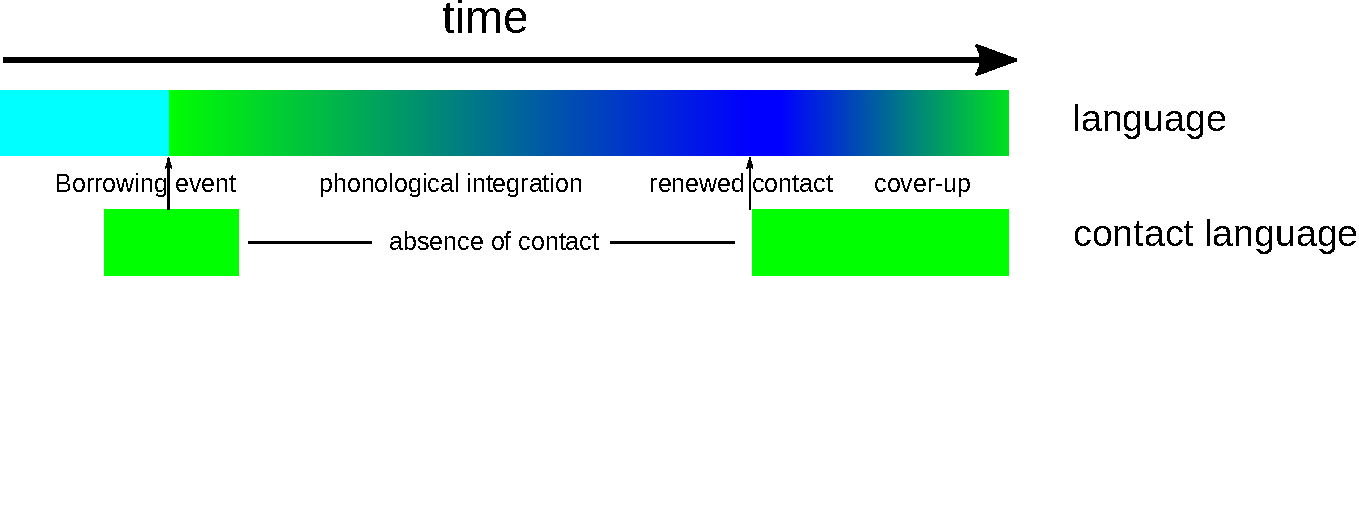
\includegraphics[width=\textwidth]{contactreversal.pdf}
  terima kasih $\to$ (\textsubbridge{t}ri$_\mu$i$_\mu$)<ma> (ka$_\mu$a$_\mu$)<si>

  `thank you'
}

\printbibliography
\end{document}
